\documentclass[11pt]{article}

% ---------------------------------------------------------------------------
% Portable preamble only (no tcolorbox/mdframed): matches the packages that
% compiled the project manuscript, so this builds on Overleaf / MiKTeX / TeX Live
% in a single pdflatex pass.
% ---------------------------------------------------------------------------
\usepackage[utf8]{inputenc}
\usepackage[T1]{fontenc}
\usepackage{lmodern}
\usepackage[margin=1in]{geometry}
\usepackage{amsmath,amssymb}
\usepackage{graphicx}
\usepackage{booktabs}
\usepackage{caption}
\usepackage{microtype}
\usepackage{xcolor}
\usepackage{framed}
\usepackage{enumitem}
\usepackage{listings}
\usepackage[hidelinks]{hyperref}

\graphicspath{{../figures/}{figures/}}

% --- coloured, page-breakable callout boxes (framed + xcolor only) ----------
\newenvironment{callout}[2][blue]{%
  \par\smallskip\colorlet{shadecolor}{#1!7}%
  \begin{shaded}\noindent{\color{#1!55!black}\bfseries #2.\ }\ignorespaces}%
  {\end{shaded}\smallskip}

\newcommand{\code}[1]{\texttt{#1}}
\newcommand{\fam}[1]{\textsf{#1}}

% --- light Python listing style ---------------------------------------------
\definecolor{codekw}{RGB}{0,90,160}
\definecolor{codestr}{RGB}{160,60,40}
\definecolor{codecmt}{RGB}{110,110,110}
\lstset{
  language=Python, basicstyle=\ttfamily\small, keywordstyle=\color{codekw},
  stringstyle=\color{codestr}, commentstyle=\color{codecmt}\itshape,
  numbers=none, breaklines=true, showstringspaces=false, frame=single,
  rulecolor=\color{black!25}, columns=fullflexible, keepspaces=true,
  xleftmargin=6pt, aboveskip=6pt, belowskip=6pt
}

\title{\vspace{-1.2cm}\textbf{Cross-Chemistry Gelation Transfer}\\[2pt]
  \large A guided, from-scratch walkthrough of the whole project ---\\
  the science, the code, the statistics, the figures, and the decisions}
\author{Personal study guide}
\date{\today}

\begin{document}
\maketitle
\vspace{-0.7cm}

\begin{callout}[gray]{How to read this}
This is a learning document, not a paper. It explains \emph{every} moving part of
the \code{gelation-transfer} project from the ground up: what the science means,
why each line of the method exists, how the statistics work, what every figure is
telling you, and --- honestly --- the dead-ends and judgement calls behind the
choices. Formulas are given and every symbol is defined, but nothing is derived
from first principles; the goal is intuition you can trust. Read it front to back
once, then use the glossary (\S\ref{sec:glossary}) as a reference.
\end{callout}

\tableofcontents
\bigskip
\hrule
\bigskip

% ===========================================================================
\section{The question, in one breath}\label{sec:question}

Imagine you have taught a model to look at a molecule's 2D structure and predict
``will this form a gel?'' You train it on one \emph{family} of molecules --- say,
peptides --- and it does well. Now a chemist hands you a completely different kind
of molecule, a nucleoside, and asks: \emph{will your model still be right?} That
single question --- how well a gelation predictor \textbf{transfers across
chemical families} --- is the whole project.

\begin{callout}[teal]{Intuition}
Think of a student who aced every past-paper for \emph{organic} chemistry. That
tells you they will do well on the organic exam. It tells you almost nothing about
how they will do on a \emph{quantum mechanics} exam. ``Good within the subject you
studied'' and ``good on a subject you never studied'' are different claims. Most
published gelation models only ever report the first; this project measures the
second.
\end{callout}

\paragraph{Low-molecular-weight gelators (LMWGs).} A gel is a mostly-liquid
material that behaves like a soft solid because a tiny amount of ``gelator''
molecules self-assemble into a network that traps the solvent. \emph{Low-molecular
-weight} gelators are small molecules (not polymers) that do this. They matter for
drug delivery, tissue engineering, and sensing, but discovering new ones is
mostly trial-and-error synthesis. A reliable ``will it gel?'' predictor would save
enormous lab effort --- \emph{if} you could trust it on new chemistry.

\paragraph{The three research questions.}
\begin{description}[leftmargin=1.6em,style=nextline]
  \item[RQ1 --- How badly does transfer fail?] Quantify the accuracy/AUC drop when
    a model is tested on a family absent from its training set.
  \item[RQ2 --- Can we predict when it will fail?] Test whether a molecule's
    \emph{applicability-domain distance} (how far it sits from the training data)
    explains the off-family mistakes.
  \item[RQ3 --- Do expensive descriptors help?] Compare commercial molecular
    descriptors (alvaDesc) against free, open-source ones.
\end{description}

\begin{callout}[blue]{Key idea}
The project's value is not a clever new algorithm. It is an \textbf{honest,
reproducible benchmark} that uses only standard, well-understood tools
(scikit-learn, RDKit, cross-validation, published applicability-domain measures)
and reports a clear, defensible finding --- including where the finding is weak.
\end{callout}

% ===========================================================================
\section{From molecules to numbers: the data}\label{sec:data}

Machine learning needs numbers, but chemistry gives us structures. The pipeline
from ``a drawn molecule'' to ``a labelled row in a table'' is where most of the
honesty of a study lives, so we spend real care here.

\subsection{SMILES: a molecule as a string}
A \textbf{SMILES} string is a compact text encoding of a molecular graph. For
example ethanol is \code{CCO} (carbon--carbon--oxygen, hydrogens implied). The
same molecule can be written many ways, so before comparing molecules we
\emph{canonicalise}: run every structure through one deterministic algorithm so
that identical molecules always produce the identical string.

\subsection{Standardisation --- making molecules comparable}
Two databases can encode ``the same'' molecule differently: one as a salt, one
neutral; one with an odd fragment attached. If we do not fix this, the same
compound looks like two different rows. Every molecule in this project passes
through the identical RDKit pipeline:
\begin{enumerate}[leftmargin=1.6em]
  \item \textbf{Parse} the SMILES; if RDKit cannot read it, drop it and log it.
  \item \textbf{Largest fragment}: keep the biggest organic piece, discarding
    counter-ions and salts (a sodium ion is not part of ``the gelator'').
  \item \textbf{Neutralise} charges where chemically sensible.
  \item \textbf{Canonicalise} to an isomeric SMILES (keeping stereochemistry).
    This canonical string becomes the \emph{identity} of the molecule.
\end{enumerate}

\begin{callout}[teal]{Intuition}
Standardisation is like normalising names before you check a guest list: ``Dr.\
Jane Q.\ Smith'', ``jane smith'', and ``Smith, Jane'' should all resolve to one
person before you look for duplicates. The canonical SMILES is that single
normalised name.
\end{callout}

\subsection{Building peptides from their sequence}
Two of our families are peptides, given as one-letter sequences (e.g.\ \code{FFG}
for Phe--Phe--Gly). RDKit's \code{MolFromSequence} builds the full chemical
structure directly from the sequence, which we then standardise like any other
molecule. This is exact and deterministic --- no manual drawing, no transcription
errors.

\subsection{The three families}
The benchmark needs several distinct chemical families. After a wide search
(\S\ref{sec:decisions}), three cleanly-deposited datasets survived:

\begin{center}
\begin{tabular}{lrrll}
\toprule
family & $n$ & gel / non-gel & label origin & chemistry \\
\midrule
\fam{nucleoside}   & 71  & 38 / 33  & experimental hydrogelation & ribose + nucleobase \\
\fam{tripeptide}   & 600 & 179 / 421 & simulated aggregation (AP $\geq 1.5$) & bare tripeptides \\
\fam{peptide\_expt}& 367 & 248 / 119 & experimental self-assembly & variable-length peptides \\
\bottomrule
\end{tabular}
\end{center}

\begin{callout}[orange]{Honesty note (a real limitation)}
These span \emph{two} core chemistries --- nucleosides versus peptides --- not
three unrelated ones. The two peptide sets differ in how they were labelled
(simulation vs experiment) and in length, but they are still peptides. We say this
plainly rather than dressing it up. It even turns out to \emph{help} RQ2 by giving
a \emph{range} of ``distances'' between families: a big chemistry gap (nucleoside
$\leftrightarrow$ peptide) and a smaller one (tripeptide $\leftrightarrow$
peptide\_expt).
\end{callout}

\subsection{Turning a continuous score into a label (the tripeptide threshold)}
The tripeptide family does not come with ``gel / non-gel'' labels. It comes from a
famous coarse-grained molecular-dynamics screen that assigned every one of the
8000 possible tripeptides an \textbf{aggregation propensity} (AP) --- a number
where higher means ``more likely to clump and self-assemble.'' To get a binary
label we must choose a threshold.

We use $\text{AP} \geq 1.5 \Rightarrow$ ``self-assembling.'' The value 1.5 is used
in the self-assembly literature to mark strong aggregators, and here it yields a
sensible $\sim$30\% positive rate. Because a threshold is a modelling choice, the
config also records a \emph{sensitivity} pair (1.4 and 1.6) so the finding can be
re-checked at nearby cuts.

\begin{callout}[teal]{Intuition}
Binarising a continuous score is like deciding a pass mark. Where you draw the
line changes how many ``pass,'' so an honest study states the line, justifies it,
and shows the conclusion does not hinge on a lucky choice.
\end{callout}

\subsection{Why we subsample the tripeptides}
The full tripeptide screen has 8000 molecules; the others have 71 and 367. If we
kept all 8000, that one family would dominate every comparison, and computing
thousands of expensive descriptors (Mordred, and your alvaDesc trial) would be
heavy. So we take a \textbf{seeded, label-stratified subsample of 600}:
``stratified'' means it preserves the $\sim$30/70 class ratio, and ``seeded''
means the same 600 are drawn every run (reproducibility). The full 8000 stay on
disk as provenance.

\subsection{Deduplication and collisions}
Within each family we drop repeated canonical SMILES. Across families we also
check: if the \emph{same} molecule appears in two families, it is assigned to one
(the earlier one in a fixed order) and the collision is counted. Exactly one such
collision occurred (a tripeptide that also appears in the experimental peptide
set). The final table \code{gelation\_all.csv} has one row per unique molecule with
columns \code{id, smiles, label, family, source\_doi}.

\begin{callout}[violet]{Analogy}
Deduplication across families is like merging two mailing lists: if the same
person is on both, you must decide which list ``owns'' them, and record that you
made that call --- otherwise your ``two independent audiences'' secretly overlap,
and any comparison between them is contaminated.
\end{callout}

\subsection{Provenance as a first-class citizen}
Every source's DOI, licence, download hash (SHA-256), and curation choices are
written to \code{PROVENANCE.md} and \code{data/raw/manifest.json}. This is not
bureaucracy: it is what lets someone (including future-you) trust that the numbers
came from where you say, under a licence that permits the use.

% ===========================================================================
\section{Turning structure into features}\label{sec:features}

A model cannot read a molecular graph directly; we must convert each molecule into
a fixed-length vector of numbers --- a \textbf{representation}. We compute four,
because RQ3 asks whether the choice matters.

\begin{description}[leftmargin=1.6em,style=nextline]
  \item[RDKit 2D descriptors (217 numbers).] Human-interpretable physicochemical
    quantities: molecular weight, number of rings, polarity estimates, counts of
    functional groups, and so on. Think ``a spec sheet of the molecule.''
  \item[Morgan / ECFP4 fingerprint (2048 bits).] A different philosophy: look at
    every atom, describe its circular neighbourhood out to two bonds, hash each
    such substructure into one of 2048 slots, and set that bit to 1. The vector
    says ``these local substructures are present.'' It captures \emph{what the
    molecule is built from} rather than bulk properties.
  \item[Mordred 2D (1613 numbers).] A large open-source descriptor set --- more of
    the ``spec sheet'' idea, much wider.
  \item[alvaDesc (4215 numbers).] A commercial descriptor package. Same spirit as
    RDKit/Mordred but proprietary; RQ3 asks if paying for it buys anything.
\end{description}

\begin{callout}[teal]{Intuition: descriptors vs fingerprints}
Descriptors are like describing a house by its \emph{statistics} (floor area,
number of windows, energy rating). A fingerprint is like listing which
\emph{building blocks} it contains (this kind of brick, that kind of door). Both
describe the house; they fail and succeed in different ways, which is exactly why
we test several.
\end{callout}

\paragraph{ECFP4, a little more concretely.} ``ECFP4'' means Extended-Connectivity
FingerPrint with diameter 4 (radius 2 bonds). For each atom you grow a small
neighbourhood, radius 0, then 1, then 2, and record an identifier for each. All
those identifiers are folded into a fixed 2048-bit vector. Two molecules sharing
many bits share many local substructures. This same fingerprint later powers the
``structural novelty'' distance in \S\ref{sec:ad}.

\paragraph{An aligned loader that fails loudly.} A subtle bug source: if a feature
table is missing a molecule, silent misalignment can shuffle labels against the
wrong rows. The loader therefore \emph{refuses to guess}: it reindexes every
feature table to the exact dataset order and raises an error naming any missing
molecule. ``Fail loudly'' beats ``fail silently'' every time in data work.

% ===========================================================================
\section{The models}\label{sec:models}

Three standard classifiers, deliberately not exotic:
\begin{description}[leftmargin=1.6em,style=nextline]
  \item[Logistic regression (primary).] Draws the best straight boundary in
    feature space; outputs a probability. Simple, fast, hard to fool yourself
    with. Being the primary model keeps the story interpretable.
  \item[Random forest.] Many decision trees on random subsets, votes averaged.
    Captures non-linear interactions.
  \item[HistGradientBoosting.] Trees built in sequence, each fixing the previous
    one's errors. Often strong on tabular data.
\end{description}

Because some families are imbalanced (e.g.\ tripeptides are 30/70), the models use
\code{class\_weight="balanced"}, which tells the model to care proportionally more
about the rarer class so it does not just predict the majority.

\begin{callout}[violet]{Analogy}
\code{class\_weight="balanced"} is like a teacher who weights a rare exam topic
more heavily so students cannot pass by ignoring it. Without it, a model can score
70\% on a 30/70 split by always saying ``no'' --- impressive-looking and useless.
\end{callout}

% ===========================================================================
\section{The honest evaluation protocol}\label{sec:protocol}

This section is the scientific heart of the project. A gelation model is easy to
\emph{seem} good; the work is in measuring it without fooling yourself.

\subsection{Data leakage: the cardinal sin}
\textbf{Leakage} is when information from the test data sneaks into training. The
classic example: you look at \emph{all} your data to decide which features are
useful, \emph{then} cross-validate using those features. The feature-selection
step already peeked at the test folds, so your score is optimistically inflated.

\begin{callout}[red]{Pitfall}
Any data-dependent step --- scaling, imputing missing values, dropping constant
columns, selecting features, choosing hyperparameters --- must be fit using
\emph{only} the training rows of the current fold. Do it on the full dataset
first and you have leaked, even though no single line of code looks obviously
wrong.
\end{callout}

\subsection{Making leak-freedom structural, not a matter of willpower}
Rather than \emph{remembering} to be careful, the code makes leakage
\emph{impossible} by construction. Every step lives inside a scikit-learn
\code{Pipeline}, and the pipeline is what gets fit on each training fold:

\begin{lstlisting}
Pipeline([
    ("clean",    CleanInf()),                 # +/-inf -> NaN
    ("impute",   SimpleImputer("median")),    # fill missing values
    ("variance", VarianceThreshold(0.0)),     # drop constant columns
    ("select",   SelectKBest(f_classif, k=200)),  # keep the 200 most
                                              # label-associated features
    ("scale",    StandardScaler()),           # mean 0, variance 1
    ("winsor",   Winsorize(1e6)),             # clip extreme values
    ("clf",      LogisticRegression(...)),    # the model
])
\end{lstlisting}

Because the \emph{whole} pipeline is fit inside each fold (wrapped by
\code{GridSearchCV} for hyperparameters), the imputer's medians, the variance
filter, the feature selection, and the scaler's mean/variance are all learned from
training rows only. Each step, in plain words:

\begin{description}[leftmargin=1.6em,style=nextline]
  \item[CleanInf] Some descriptors return $\pm\infty$; convert to ``missing'' so
    the imputer can handle them uniformly.
  \item[SimpleImputer(median)] Replace missing values with the column median
    (robust to outliers).
  \item[VarianceThreshold] A column that never changes carries no information and
    breaks some later maths; drop it.
  \item[SelectKBest($f\_classif$)] Keep the $k$ features most statistically
    associated with the label, scored by a one-way ANOVA $F$-test. Intuition: the
    $F$ statistic is large when a feature's mean differs a lot between gel and
    non-gel relative to its spread within each class.
  \item[StandardScaler] Put every feature on the same scale so, e.g., molecular
    weight (hundreds) does not dwarf a 0/1 flag. Essential for logistic regression.
  \item[Winsorize] Clip standardised values to $\pm 10^6$. This is a safety guard
    with an interesting backstory (\S\ref{sec:overflow}).
\end{description}

\subsection{Nested cross-validation}
We need two different things from our data: to \emph{choose} hyperparameters, and
to \emph{estimate} performance honestly. Using the same split for both leaks. So
we nest:
\begin{itemize}[leftmargin=1.6em]
  \item An \textbf{outer} loop splits the family into train/test folds; the test
    fold is used \emph{only} to score.
  \item An \textbf{inner} loop (inside \code{GridSearchCV}) splits the outer-train
    data again to pick the best hyperparameters.
\end{itemize}

\begin{callout}[violet]{Analogy}
Nested CV is the difference between the questions you \emph{practise} on and the
questions on the \emph{real exam}. The inner loop is practice (tune your
approach); the outer loop is the sealed exam (measure how you actually do). Reuse
the exam as practice and your reported grade is a lie.
\end{callout}

\paragraph{Repeated, stratified, pooled.} The outer loop is a
\emph{repeated stratified} 5$\times$10 cross-validation: 5 folds, repeated 10
times with different shuffles; ``stratified'' keeps the class ratio in every fold.
Each molecule is predicted many times (once per repeat); we average its predicted
probability, giving one honest ``out-of-fold'' prediction per molecule.

\subsection{Scoring: accuracy, AUC, and the baseline you must always print}
\begin{description}[leftmargin=1.6em,style=nextline]
  \item[Accuracy] fraction correct at a 0.5 probability cutoff. Easy to read, but
    misleading under class imbalance.
  \item[ROC--AUC] the probability that the model ranks a random positive above a
    random negative. $0.5$ is a coin flip; $1.0$ is perfect. It is threshold-free,
    which is why it is our main metric.
  \item[Majority baseline] the accuracy of always predicting the commoner class.
    We print it next to every score, because ``82\% accurate'' means one thing at
    a 50/50 split and nothing at an 82/18 split.
\end{description}

\begin{callout}[teal]{Intuition: what AUC really measures}
Pick one gel and one non-gel molecule at random. AUC is the chance the model gives
the gel the higher score. That is why AUC $<0.5$ is meaningful and alarming: it
means the model systematically ranks them the \emph{wrong} way round --- worse
than guessing (we will see exactly this in transfer, \S\ref{sec:transfer}).
\end{callout}

\subsection{Confidence intervals by bootstrapping over molecules}
A single AUC number hides its uncertainty. We estimate that uncertainty by the
\textbf{bootstrap}: resample the molecules with replacement many times (here
2000), recompute the metric each time, and take the 2.5th and 97.5th percentiles
as a 95\% interval.

\begin{callout}[red]{Pitfall (subtle but important)}
We resample \emph{molecules}, not \emph{folds}. Resampling folds would measure the
noise of the CV splitter; resampling molecules measures what we actually care
about --- how much the estimate would wobble if we had drawn a different sample of
molecules from the same chemistry.
\end{callout}

\subsection{The leakage-guard test: proving the pipeline is honest}
Claims of leak-freedom are cheap; the project \emph{tests} it. Construct a
synthetic dataset of pure noise (no real signal) plus, in one variant, a single
genuinely predictive feature. Then:
\begin{itemize}[leftmargin=1.6em]
  \item Select features on \emph{all} the data, then cross-validate: the noise-only
    AUC jumps well above 0.5 --- \emph{that is leakage made visible}.
  \item Select \emph{inside} the pipeline (our way): the noise-only AUC stays near
    0.5 --- no leak --- yet it still finds the genuinely predictive feature when
    one exists. So the pipeline is neither leaky nor inert.
\end{itemize}
This single test is worth more than any amount of assurance in a comment.

% ===========================================================================
\section{Transfer: does the model survive new chemistry?}\label{sec:transfer}

\subsection{The design (always split by family)}
Two experiments, and the golden rule is to \textbf{split by family}, never by
random shuffle across families --- because the whole question is about crossing
the family boundary.
\begin{description}[leftmargin=1.6em,style=nextline]
  \item[Pairwise matrix] Train on all of family A, test on all of family B, for
    every ordered pair. The diagonal (A$\to$A) is filled with the honest
    within-family cross-validated score, not a train-equals-test number.
  \item[Leave-one-family-out (LOFO)] Train on the union of every family but one,
    test on the held-out family. This is the realistic ``I have several known
    chemistries; will it work on a new one?'' scenario.
\end{description}

\subsection{The result: transfer collapses}
Figure~\ref{fig:heatmap} is the story in one picture.

\begin{figure}[h]
\centering
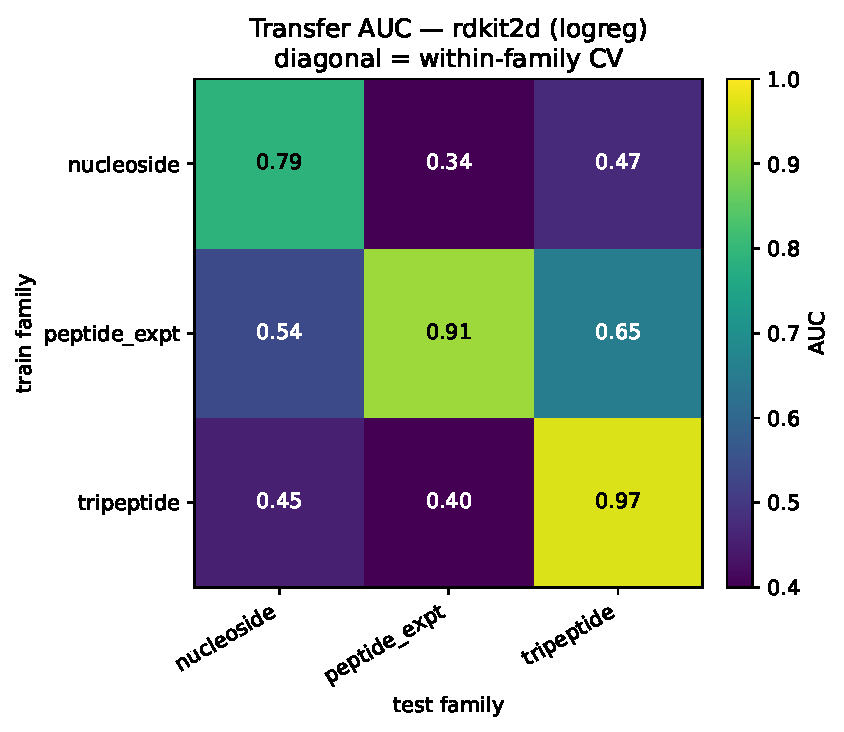
\includegraphics[width=0.72\linewidth]{fig_transfer_rdkit2d}
\caption{\textbf{Transfer AUC heat-map (RDKit-2D, logistic regression).} Rows are
the training family, columns the test family. Bright = high AUC. The diagonal
(within-family cross-validation) glows: 0.79, 0.91, 0.97. Every off-diagonal cell
(train on one chemistry, test on another) is dark --- 0.34 to 0.65 --- i.e.\ at or
below chance. Reading a single cell: ``train on nucleoside, test on peptide\_expt''
$=0.34$, which is \emph{below} 0.5, meaning the learned rule is actively
\emph{backwards} on that family.}
\label{fig:heatmap}
\end{figure}

Averaged over all descriptors and models, cross-family AUC hovers around 0.47--0.63
--- essentially a coin flip --- while within-family AUC is 0.78--0.97. The best
off-diagonal cell is peptide\_expt~$\to$~tripeptide (0.65), which makes sense: those
two are the \emph{same} broad chemistry (both peptides), the smallest gap to cross.

\begin{callout}[blue]{Key idea (RQ1 answered)}
A strong within-family score is \emph{not} evidence a gelation model will work on
new chemistry. Here it transfers no better than guessing, and sometimes
\emph{inverts} (AUC $<0.5$): a feature that means ``gel'' in nucleosides can mean
``non-gel'' in peptides, so the model confidently gets the new family backwards.
\end{callout}

\subsection{A bug that taught a lesson: the float32 overflow}\label{sec:overflow}
When we first ran transfer with tree models, it \emph{crashed}: ``input contains
infinity.'' The cause is a small chemistry-meets-numerics story worth
understanding.

Some descriptors (RDKit's \code{Ipc}, an information-content index) grow
explosively for long molecules --- the 24-residue peptides produced astronomically
large values. \emph{Within} a family this is harmless: standardising subtracts the
mean and divides by the standard deviation, and since that same huge molecule
inflates the family's own standard deviation, its standardised value stays modest.
\emph{Across} families it is not harmless: when you standardise a peptide's giant
\code{Ipc} using the \emph{nucleoside} family's tiny mean and spread, you get an
astronomically large $z$-score, which overflows the 32-bit float that the tree
models use internally.

The fix is the \code{Winsorize} step: clip standardised values to $\pm 10^6$ ---
far beyond any real $z$-score, so it never touches within-family results (verified:
identical to six decimals), but it tames the pathological cross-family values so
nothing overflows.

\begin{callout}[teal]{Intuition}
Standardisation quietly assumes the test data lives on the same scale as the
training data. Cross-family, that assumption breaks --- and the breakage showing up
as a numeric overflow is, in a sense, the applicability-domain problem
(\S\ref{sec:ad}) announcing itself in the crudest possible way.
\end{callout}

% ===========================================================================
\section{Applicability domain: knowing when to distrust a prediction}\label{sec:ad}

If transfer generally fails, the practical question becomes: can the model tell us
\emph{which} off-family predictions to distrust? The \textbf{applicability domain}
(AD) is the region of chemical space the model actually ``knows,'' and AD distance
measures how far a new molecule sits from it.

\begin{callout}[violet]{Analogy}
A weather model trained only on coastal cities can still be \emph{asked} about a
mountain town, but you should not trust it there --- the mountain is outside its
domain. AD distance is a ``how far from familiar terrain is this?'' meter attached
to each prediction.
\end{callout}

\subsection{Leverage (the hat value)}
\textbf{Leverage} measures how far a molecule sits from the centre of the training
data in descriptor space. For a training design matrix $X$ (rows = molecules,
columns = standardised descriptors) and a query row $\mathbf{x}$,
\[
  h(\mathbf{x}) \;=\; \mathbf{x}\,(X^\top X)^{-1}\mathbf{x}^\top .
\]
The \textbf{Williams threshold} $h^\ast = 3p/n$ (with $p$ descriptors and $n$
training molecules) is the conventional line above which a molecule is ``outside
the domain.'' A useful sanity fact: the average leverage of the training
molecules themselves is exactly $p/n$, so $h^\ast$ is just ``three times the
typical training leverage.''

\begin{callout}[teal]{Intuition}
Leverage is a distance-from-the-crowd score, but shaped by the training cloud:
molecules far out \emph{along directions the training set actually varies in} get
moderate leverage; molecules far out in a \emph{new} direction the training set
never explored get very high leverage. That is precisely what you want when asking
``is this outside what the model has seen?''
\end{callout}

\paragraph{A dimensionality wrinkle.} The formula needs $p<n$ (otherwise
$X^\top X$ is not invertible). alvaDesc has 4215 descriptors --- far more than the
molecules in a small family --- so when needed we first compress the descriptors
with PCA to fewer components than training molecules, then compute leverage there.
The concept is unchanged; only the coordinate system is reduced.

\subsection{Structural novelty and kNN distance}
Two more AD measures give independent views:
\begin{description}[leftmargin=1.6em,style=nextline]
  \item[Novelty $= 1 - \max$ ECFP4 Tanimoto.] The Tanimoto similarity between two
    fingerprints is (shared bits)/(bits set in either). Take a query molecule's
    \emph{highest} similarity to any training molecule, subtract from 1: novelty
    $0$ means ``a near-twin exists in training,'' novelty near $1$ means
    ``structurally unlike anything seen.''
  \item[kNN distance.] The average Euclidean distance to the $k$ nearest training
    molecules in standardised descriptor space --- a straightforward ``how far are
    my nearest neighbours?''
\end{description}

\subsection{The headline result: an AD-based trust flag works}
Now the payoff. Pool every off-family prediction and sort molecules by leverage.
Figure~\ref{fig:headline} shows accuracy falling as leverage rises.

\begin{figure}[h]
\centering
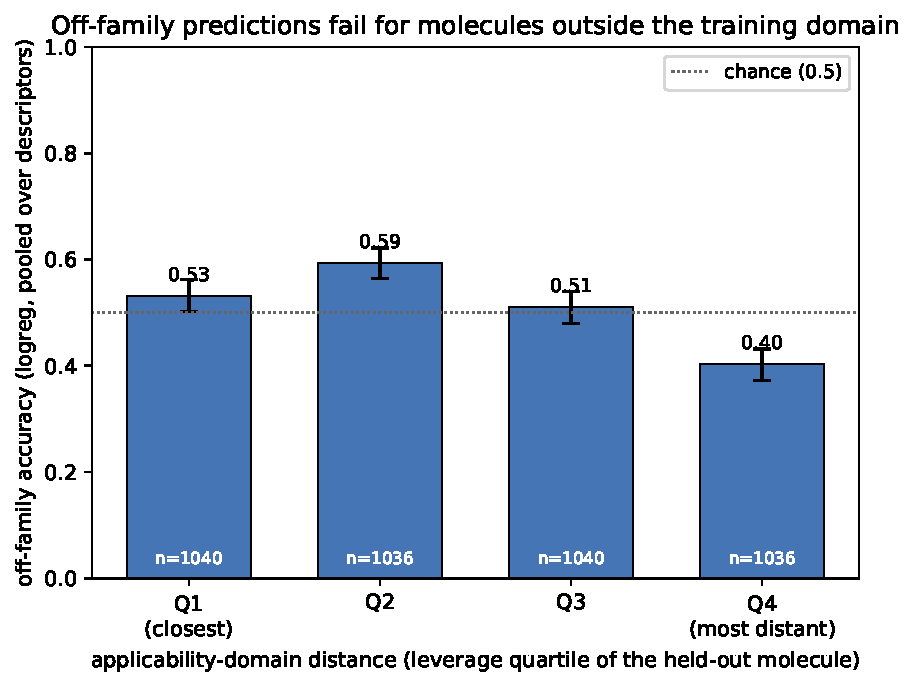
\includegraphics[width=0.72\linewidth]{fig_headline_ad_trust}
\caption{\textbf{The lead result.} Off-family predictions, grouped into leverage
quartiles from closest (Q1) to most distant (Q4). Bars are accuracy; the dotted
line is chance (0.5). Predictions for molecules \emph{near} the training domain
are near chance already; predictions for the \emph{most distant} molecules (Q4)
fall to 0.40 --- \emph{worse} than a coin flip. Split at the Williams threshold,
accuracy is 0.56 inside the domain versus 0.46 outside.}
\label{fig:headline}
\end{figure}

Statistically, molecules the model gets \emph{wrong} off-family have significantly
higher leverage (median 1.60 vs 0.96) and kNN distance (9.09 vs 7.88) than those
it gets right, each with $p\approx 10^{-10}$ by a Mann--Whitney test
(\S\ref{sec:stats}). Figure~\ref{fig:molad} shows this separation directly.

\begin{figure}[h]
\centering
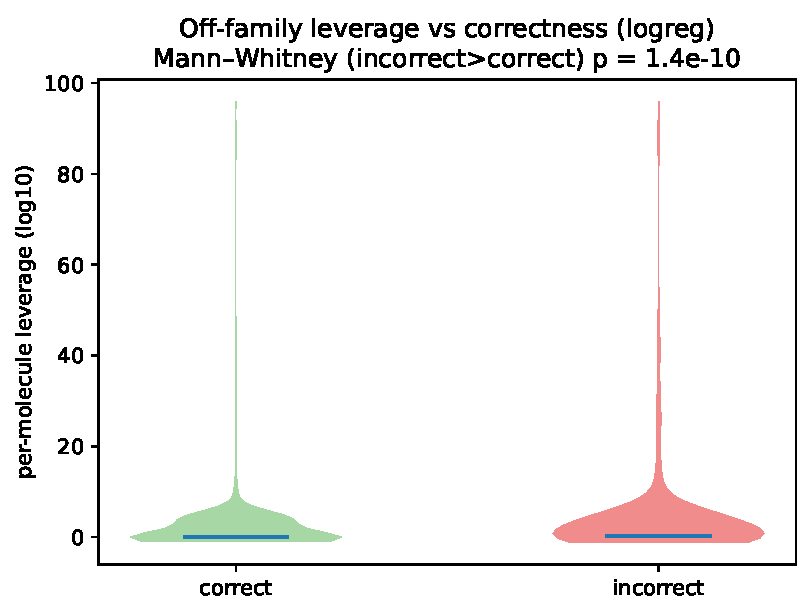
\includegraphics[width=0.62\linewidth]{fig_molecule_ad}
\caption{\textbf{Leverage of correct vs incorrect off-family predictions}
(log scale). The ``incorrect'' cloud sits clearly higher: being far outside the
training domain is associated with being wrong.}
\label{fig:molad}
\end{figure}

\begin{callout}[blue]{Key idea (RQ2 answered, at the molecule level)}
You cannot trust an off-family prediction blindly, but you \emph{can} ask how far
the molecule is from the training domain. High leverage / kNN distance flags the
likely failures. Interestingly, ECFP4 \emph{novelty} barely separates right from
wrong ($p\approx 0.24$) --- a useful negative result: fingerprint dissimilarity is
a weaker trust signal here than descriptor-space leverage.
\end{callout}

\subsection{The confound we refuse to hide}\label{sec:confound}
There is a tempting but \emph{wrong} way to make the RQ2 claim: correlate each
family's median AD distance with its performance drop. Do that and you get a
\emph{negative} correlation (Spearman $\rho\approx-0.65$) --- the opposite of the
hypothesis. Figure~\ref{fig:confound} shows why, and it is instructive.

\begin{figure}[h]
\centering
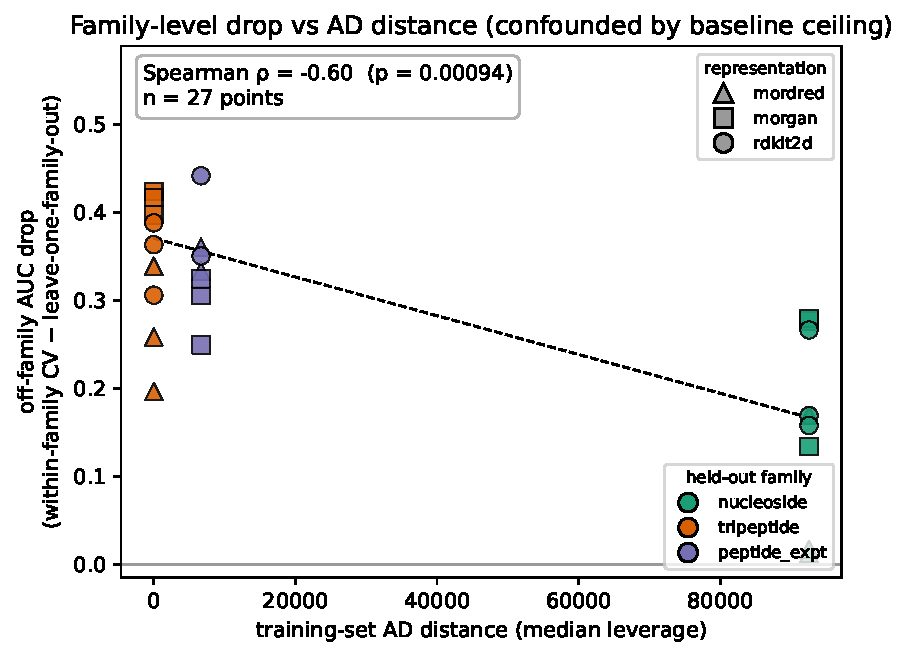
\includegraphics[width=0.66\linewidth]{fig_family_drop_vs_ad}
\caption{\textbf{Why the family-level view is misleading.} Each point is a
(family, descriptor, model). The nucleoside family is the most chemically distant
(highest AD distance) yet shows the \emph{smallest} AUC drop --- only because its
within-family score was already low (0.72), leaving little to lose. With just three
families, ``drop'' is entangled with each family's starting ceiling, so this
coarse view is shown as a caveated secondary, never the headline.}
\label{fig:confound}
\end{figure}

\begin{callout}[orange]{Honesty note}
This is the difference between a well-powered, confound-free result (thousands of
molecule-level predictions, \S\ref{fig:headline}) and an underpowered, confounded
one (three family points). A less careful write-up would report whichever sign
looked better. We report both and explain which to believe and why.
\end{callout}

\subsection{The two statistics we lean on}\label{sec:stats}
\begin{description}[leftmargin=1.6em,style=nextline]
  \item[Spearman correlation $\rho$.] Correlation of \emph{ranks} rather than raw
    values: it asks ``do larger $x$ tend to go with larger $y$?'' without assuming
    a straight-line relationship. Ranges $-1$ to $+1$; the $p$-value is the chance
    of seeing such a rank-association if there were truly none.
  \item[Mann--Whitney $U$ test.] A rank-based test of whether one group's values
    tend to be larger than another's --- here, whether ``incorrect'' molecules
    have larger leverage than ``correct'' ones --- \emph{without} assuming a normal
    distribution. Perfect for skewed quantities like leverage.
\end{description}

% ===========================================================================
\section{Do expensive descriptors help? (RQ3)}\label{sec:rq3}

Finally, the commercial-versus-open comparison. Figure~\ref{fig:desc} compares the
cross-family transfer AUC of all four representations.

\begin{figure}[h]
\centering
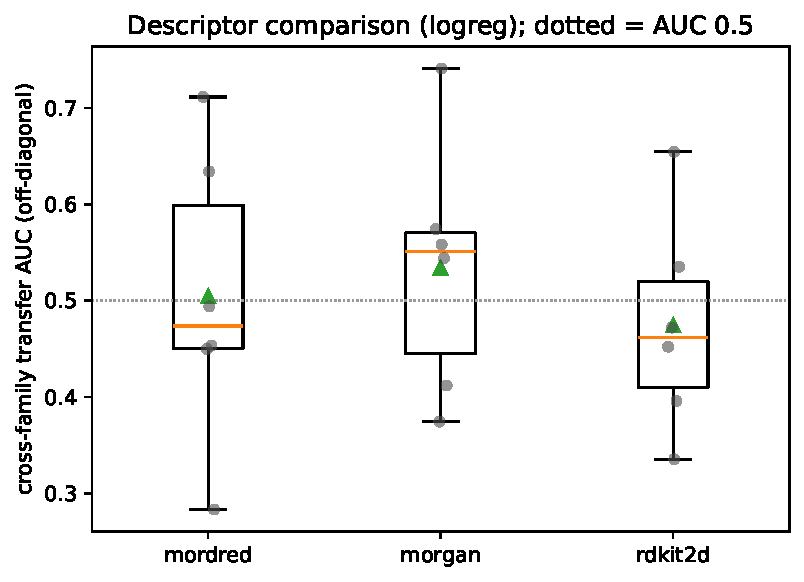
\includegraphics[width=0.66\linewidth]{fig_descriptor_comparison}
\caption{\textbf{Descriptor comparison (logistic regression).} Each box is the
spread of a representation's off-diagonal (cross-family) transfer AUCs; the green
triangle is the mean; the dotted line is chance. All four --- including commercial
\fam{alvadesc} --- sit around 0.5 with heavily overlapping boxes.}
\label{fig:desc}
\end{figure}

The mean cross-family AUCs (rows = descriptor, columns = model):

\begin{center}
\begin{tabular}{lccc}
\toprule
 & logreg & rf & hgb \\
\midrule
rdkit2d  & 0.474 & 0.576 & 0.499 \\
morgan   & 0.534 & 0.491 & 0.492 \\
mordred  & 0.504 & 0.633 & 0.566 \\
\textbf{alvadesc} & 0.495 & 0.577 & 0.524 \\
\bottomrule
\end{tabular}
\end{center}

\begin{callout}[blue]{Key idea (RQ3 answered)}
The commercial descriptors transfer no better than the free ones: alvaDesc's 4215
2D descriptors land in the same near-chance band (0.50--0.58), and its
within-family scores are on par too. Mordred+random-forest is nominally highest
(0.633) but the intervals overlap; with three families no ranking is defensible.
The honest answer is negative --- paying for descriptors does not buy
cross-chemistry transfer here.
\end{callout}

\subsection{The within-family baseline, for completeness}
Figure~\ref{fig:within} confirms the flip side: every family \emph{is} learnable
within itself, well above its majority baseline. That is what makes the transfer
collapse so striking --- the skill is real, it just does not travel.

\begin{figure}[h]
\centering
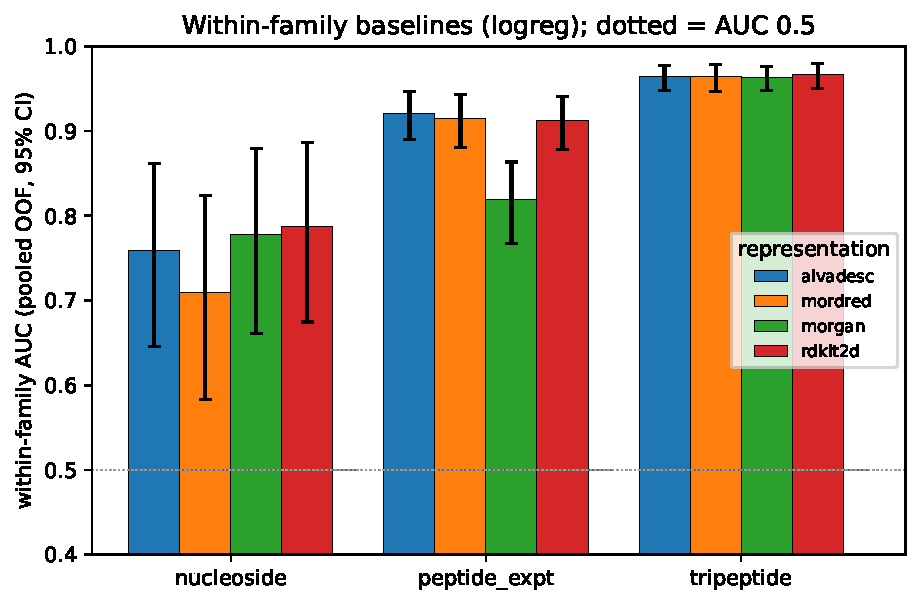
\includegraphics[width=0.72\linewidth]{fig_within_family}
\caption{\textbf{Within-family AUC with 95\% bootstrap intervals} (logistic
regression). All bars sit well above 0.5. Nucleosides are hardest ($n=71$,
AUC~$\approx0.79$); the peptide families reach 0.91--0.97.}
\label{fig:within}
\end{figure}

% ===========================================================================
\section{Reproducibility and engineering}\label{sec:repro}

Good science here is inseparable from good software hygiene.

\begin{description}[leftmargin=1.6em,style=nextline]
  \item[One config, no magic numbers.] Seeds, thresholds, CV settings, and paths
    live in \code{config.yaml}; scripts read them. Nothing important is buried in
    code.
  \item[Determinism.] One master seed feeds every random step (subsample, CV
    shuffles, model randomness), so two runs produce byte-identical result tables
    --- and a test asserts it.
  \item[Resumable runs.] Each stage skips work already in its output CSV, so a long
    grid can stop and continue without recomputation.
  \item[Tracked vs regenerable.] Small, reproducible outputs (the dataset, results
    tables, figures) are committed. Large caches that any run regenerates
    (RDKit/Morgan/Mordred matrices) are git-ignored. The alvaDesc exports are a
    special case: licence-gated and \emph{not} regenerable by open code, so they
    are documented with checksums in \code{PROVENANCE.md} rather than committed.
  \item[Tests as guardrails.] 22 tests cover data invariants, feature alignment,
    the leakage guard, the AD maths (e.g.\ $h^\ast=3p/n$, novelty $\in[0,1]$), and
    determinism. They are the difference between ``I believe it works'' and ``it is
    checked.''
\end{description}

\begin{callout}[teal]{Intuition}
Treat every result file as something a stranger must be able to regenerate from
raw data with one command. That discipline is what turns ``a script that gave a
number'' into ``a benchmark someone can trust.''
\end{callout}

% ===========================================================================
\section{Problems and decisions: how the project actually went}\label{sec:decisions}

Research is a sequence of judgement calls. The honest ones, gathered:

\begin{description}[leftmargin=1.6em,style=nextline]
  \item[No clean non-peptide family.] The plan wanted a third, clearly-distinct
    chemistry (sugars, ureas). But non-peptide gelators exist in the literature
    only as \emph{drawn structures} in review articles --- no deposited,
    machine-readable SMILES-plus-labels. Curating them by hand would have been
    subjective and error-prone. \textbf{Decision:} rather than fabricate a shaky
    family, keep three clean datasets and state honestly that they span two
    chemistries. Integrity over the appearance of breadth.
  \item[Publisher paywalls / bot-blocking.] Several candidate datasets sat behind
    sites that block automated access. \textbf{Decision:} do not attempt to bypass
    protections; use only cleanly-deposited, licence-clear sources (a GitHub
    deposit for the peptides, the sibling reproduction for the nucleosides).
  \item[The AP threshold.] Binarising a continuous simulation score at 1.5 is a
    choice; \textbf{decision:} justify it from the literature and record a
    sensitivity pair so the conclusion can be re-checked.
  \item[The tripeptide subsample.] 8000 vs 71 would swamp every comparison and
    balloon compute. \textbf{Decision:} a seeded, stratified 600 --- ``simple and
    correct'' over ``use everything and hope.''
  \item[The float32 overflow.] A real crash (\S\ref{sec:overflow}) from pathological
    descriptors under cross-family standardisation. \textbf{Decision:} a
    leak-free winsorize step, verified to be a no-op within families so existing
    baselines stand.
  \item[The AD confound.] The tidy ``drop vs distance'' story had the wrong sign
    (\S\ref{sec:confound}). \textbf{Decision:} demote it to a caveated secondary
    and lead with the well-powered molecule-level result.
\end{description}

\begin{callout}[orange]{The meta-lesson}
Every one of these was a fork where the ``looks more impressive'' path and the
``more honest'' path diverged. A benchmark is only worth something if it takes the
honest fork every time --- and says so out loud.
\end{callout}

% ===========================================================================
\section{Glossary}\label{sec:glossary}

\begin{description}[leftmargin=1.6em,style=nextline,itemsep=1pt]
  \item[LMWG] Low-molecular-weight gelator --- a small molecule that self-assembles
    to gel a solvent.
  \item[SMILES] A text string encoding a molecule's structure.
  \item[Canonicalisation] Producing one deterministic SMILES per molecule so
    identical molecules match.
  \item[Descriptor] A number summarising a molecular property (weight, rings,
    polarity, \dots).
  \item[Fingerprint (ECFP4)] A bit-vector recording which local substructures a
    molecule contains.
  \item[Tanimoto] Similarity between two fingerprints: shared bits over union of
    set bits.
  \item[AP] Aggregation propensity --- a simulated self-assembly score for the
    tripeptides.
  \item[Leakage] Test information contaminating training, inflating scores.
  \item[Pipeline] A chain of steps fit together inside each fold to prevent leakage.
  \item[Nested CV] Inner loop tunes hyperparameters; outer loop estimates
    performance.
  \item[Stratified] A split that preserves the class ratio.
  \item[OOF] Out-of-fold: a molecule's prediction from a fold in which it was
    \emph{not} used for training.
  \item[AUC] Probability the model ranks a random positive above a random negative;
    0.5 is chance.
  \item[Majority baseline] Accuracy of always predicting the commoner class.
  \item[Bootstrap] Resampling with replacement to estimate uncertainty.
  \item[Transfer] Training on one family, testing on another.
  \item[LOFO] Leave-one-family-out: train on all families but one, test on it.
  \item[Applicability domain (AD)] The region of chemical space a model can be
    trusted in.
  \item[Leverage] $h=\mathbf{x}(X^\top X)^{-1}\mathbf{x}^\top$; distance from the
    training centre; threshold $h^\ast=3p/n$.
  \item[Novelty] $1-\max$ Tanimoto to the training set.
  \item[Winsorize] Clipping extreme values to a bound.
  \item[Spearman $\rho$] Rank correlation.
  \item[Mann--Whitney $U$] Rank test for whether one group's values exceed
    another's.
\end{description}

% ===========================================================================
\section{What to take away}\label{sec:takeaway}

\begin{enumerate}[leftmargin=1.6em]
  \item \textbf{Within-family accuracy is not transferable evidence.} A gelation
    model that scores AUC 0.9+ on its own chemistry can be a coin flip --- or worse
    --- on a chemistry it never saw.
  \item \textbf{But the model can flag its own blind spots.} Applicability-domain
    distance (leverage, nearest-neighbour distance) reliably marks the off-family
    predictions most likely to be wrong; use it as a ``trust this?'' meter. Plain
    structural novelty is a weaker guide.
  \item \textbf{Expensive descriptors are not a shortcut.} Commercial alvaDesc did
    not transfer better than free RDKit/Morgan/Mordred descriptors.
  \item \textbf{Honesty is a method, not a mood.} The leak-free pipeline, the
    printed baselines, the stated threshold and its sensitivity, the demoted
    confound, and the two-chemistries caveat are what make the negative result
    credible. A small honest finding beats an oversold one.
\end{enumerate}

\begin{callout}[blue]{One sentence to remember}
Before you trust a gelation prediction on a new scaffold, check how far that
molecule sits from the training set's applicability domain --- because far outside
it, the model's confidence is not evidence.
\end{callout}

\end{document}
